\documentclass[12pt,a4paper]{article}

% Pakiety językowe i kodowanie
\usepackage[utf8]{inputenc}
\usepackage[T1]{fontenc}
\usepackage[polish]{babel}

% Pakiety matematyczne i graficzne
\usepackage{amsmath}
\usepackage{amsfonts}
\usepackage{amssymb}
\usepackage{graphicx}
\usepackage{float}
\usepackage{geometry}

% Nieco mniejsze marginesy dla lepszego dopasowania
\geometry{margin=2.0cm}

\title{Sprawozdanie: Rozwiązywanie liniowych równań rekurencyjnych}
\author{Franciszek Szarek, 183962}
\date{\today}

\begin{document}

\maketitle

\tableofcontents
\clearpage

\section{Wprowadzenie}
Celem niniejszego sprawozdania jest analiza oraz weryfikacja analitycznych rozwiązań liniowych równań rekurencyjnych: jednorodnego oraz niejednorodnego. Obliczenia wykonane ręcznie zostały zweryfikowane za pomocą systemu algebry komputerowej Maxima (pakiet \texttt{solve\_rec}) oraz zilustrowane na wykresie w programie Gnuplot.

\section{Równanie rekurencyjne jednorodne}

Pierwszym etapem było rozwiązanie jednorodnego równania rekurencyjnego postaci:
\begin{equation}
    a_n = 10a_{n-1} + 17a_{n-2}
\end{equation}
z warunkami początkowymi $a_1 = 0$ oraz $a_2 = 9$.

\begin{figure}[H]
    \centering
    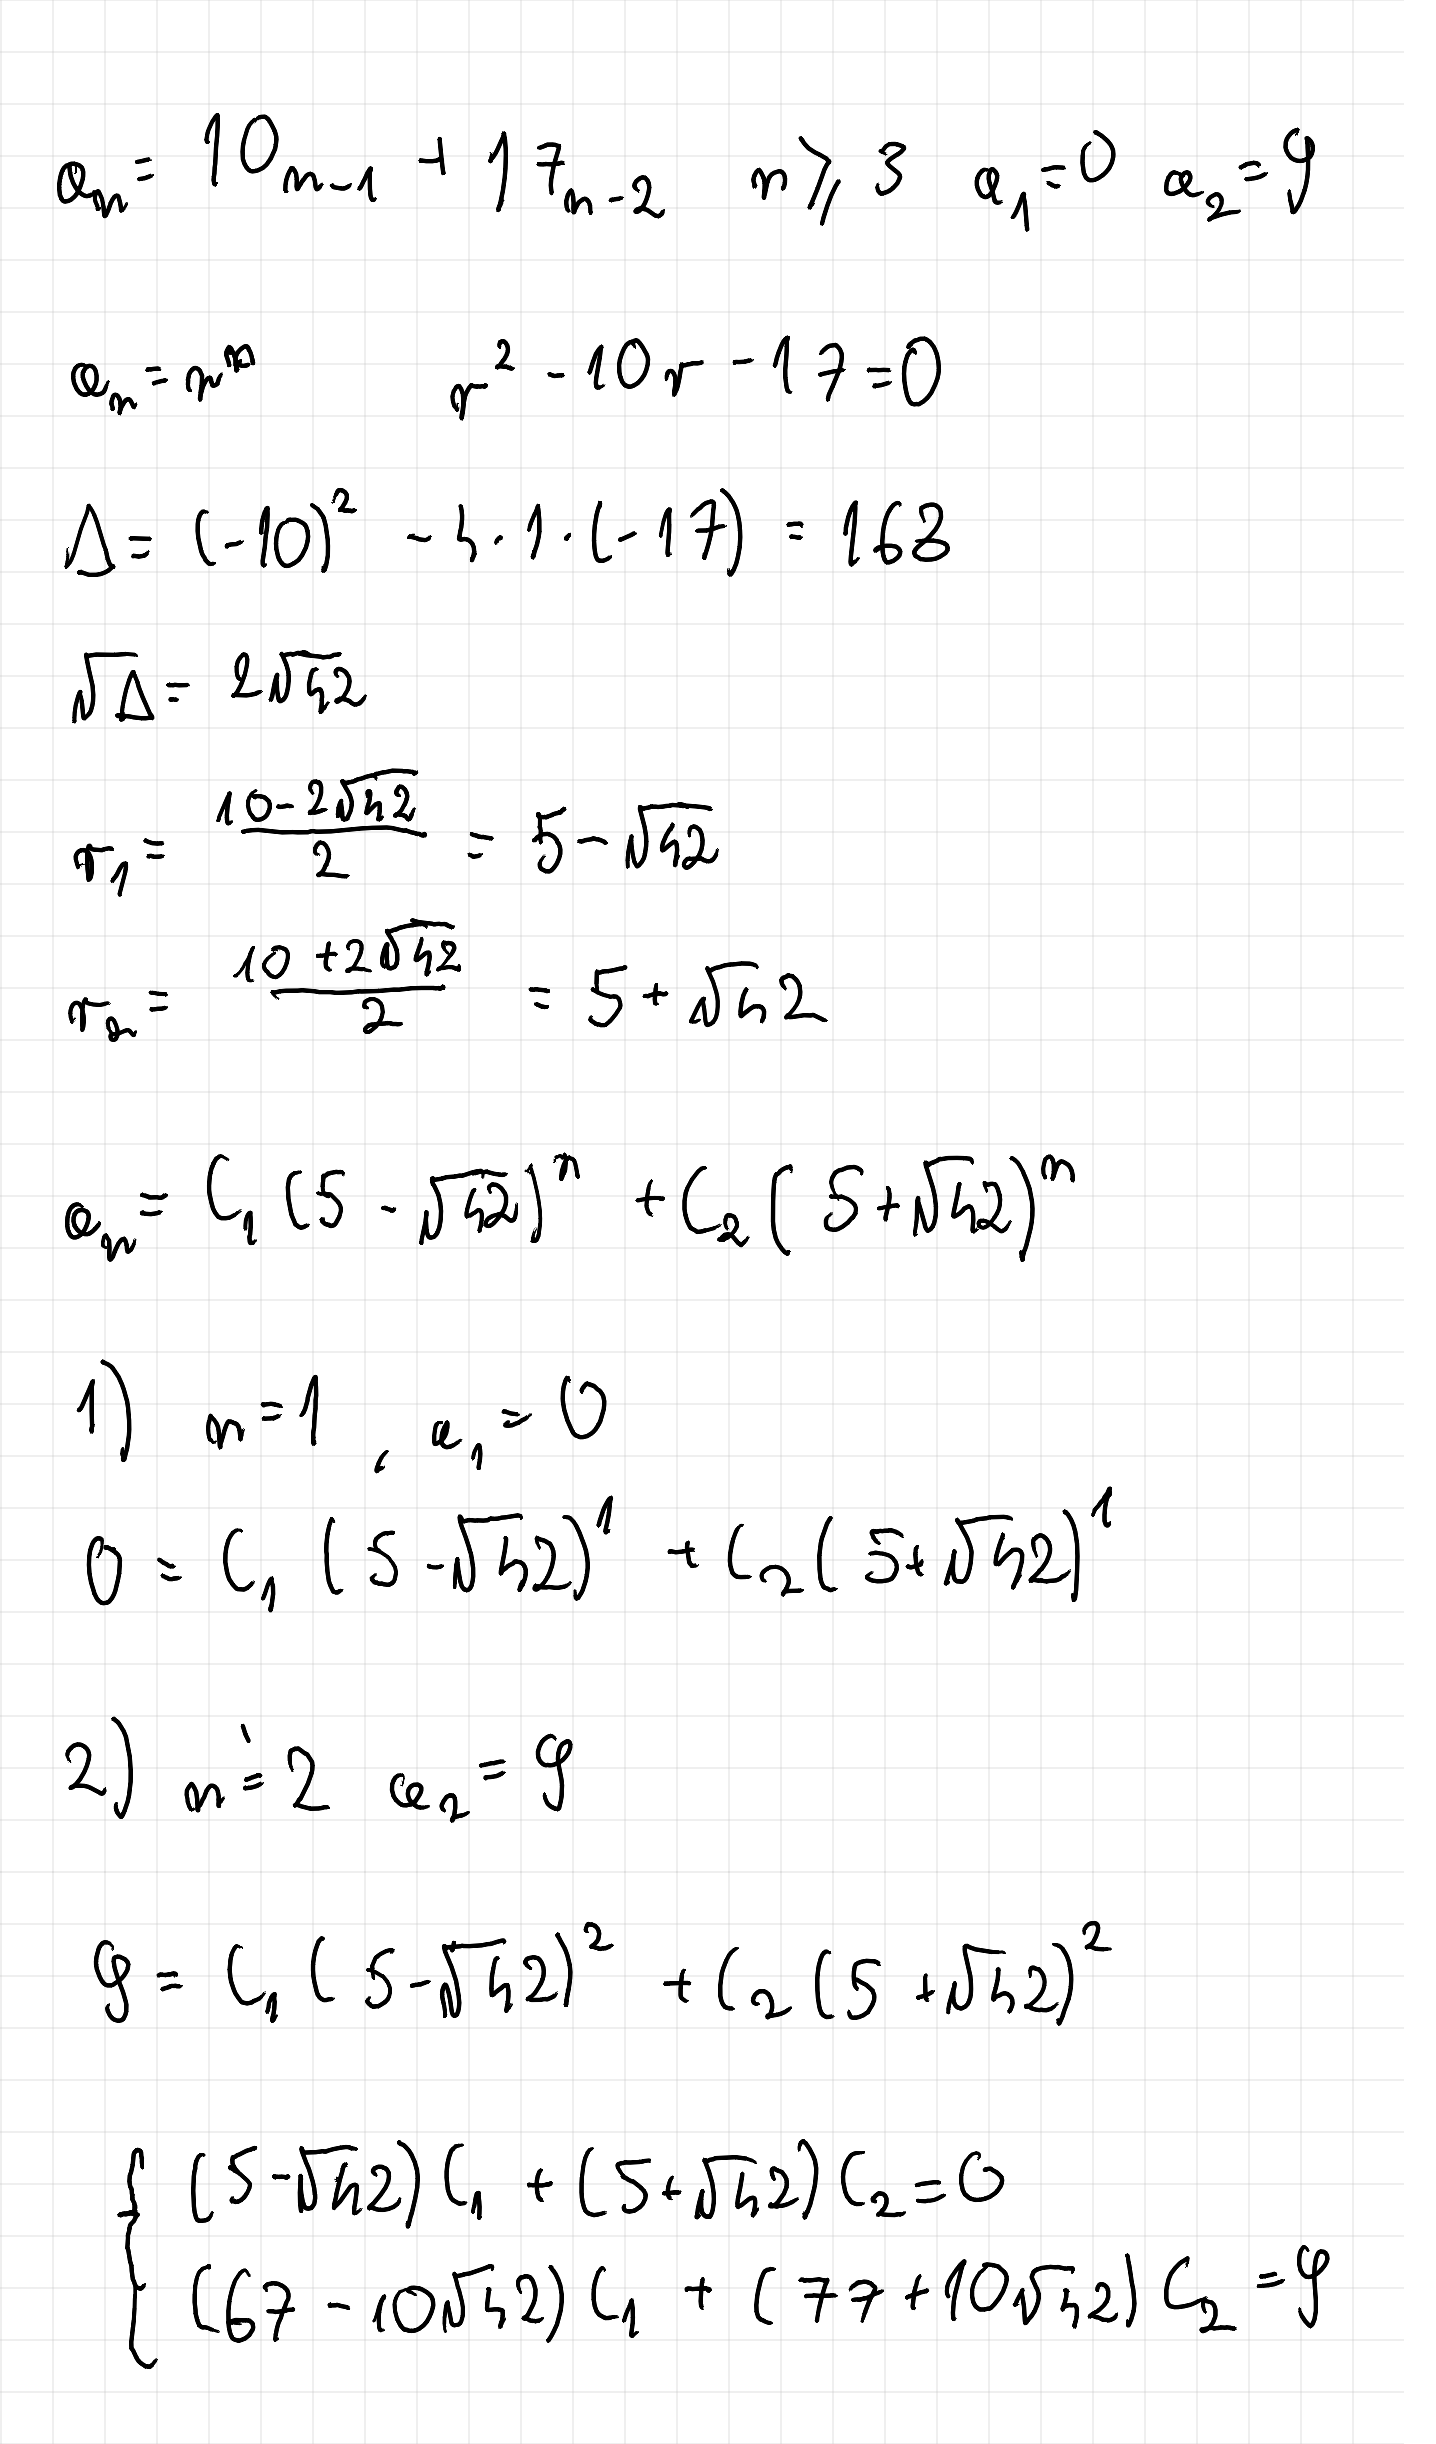
\includegraphics[width=0.65\textwidth]{jednorodne.png}
    \caption{Równanie charakterystyczne i układ równań dla warunków początkowych.}
    \label{fig:jednorodne_1}
\end{figure}

\textbf{Opis do Rysunku \ref{fig:jednorodne_1}:}
W pierwszej części obliczeń wyznaczono równanie charakterystyczne $r^2 - 10r - 17 = 0$. Następnie obliczono wyróżnik $\Delta = 168$ i pierwiastki $r_1 = 5 - \sqrt{42}$ oraz $r_2 = 5 + \sqrt{42}$. Zapisano postać ogólną rozwiązania, a po podstawieniu warunków początkowych ($n=1, a_1=0$ oraz $n=2, a_2=9$) ułożono układ równań z dwiema niewiadomymi $C_1$ i $C_2$.

\begin{figure}[H]
    \centering
    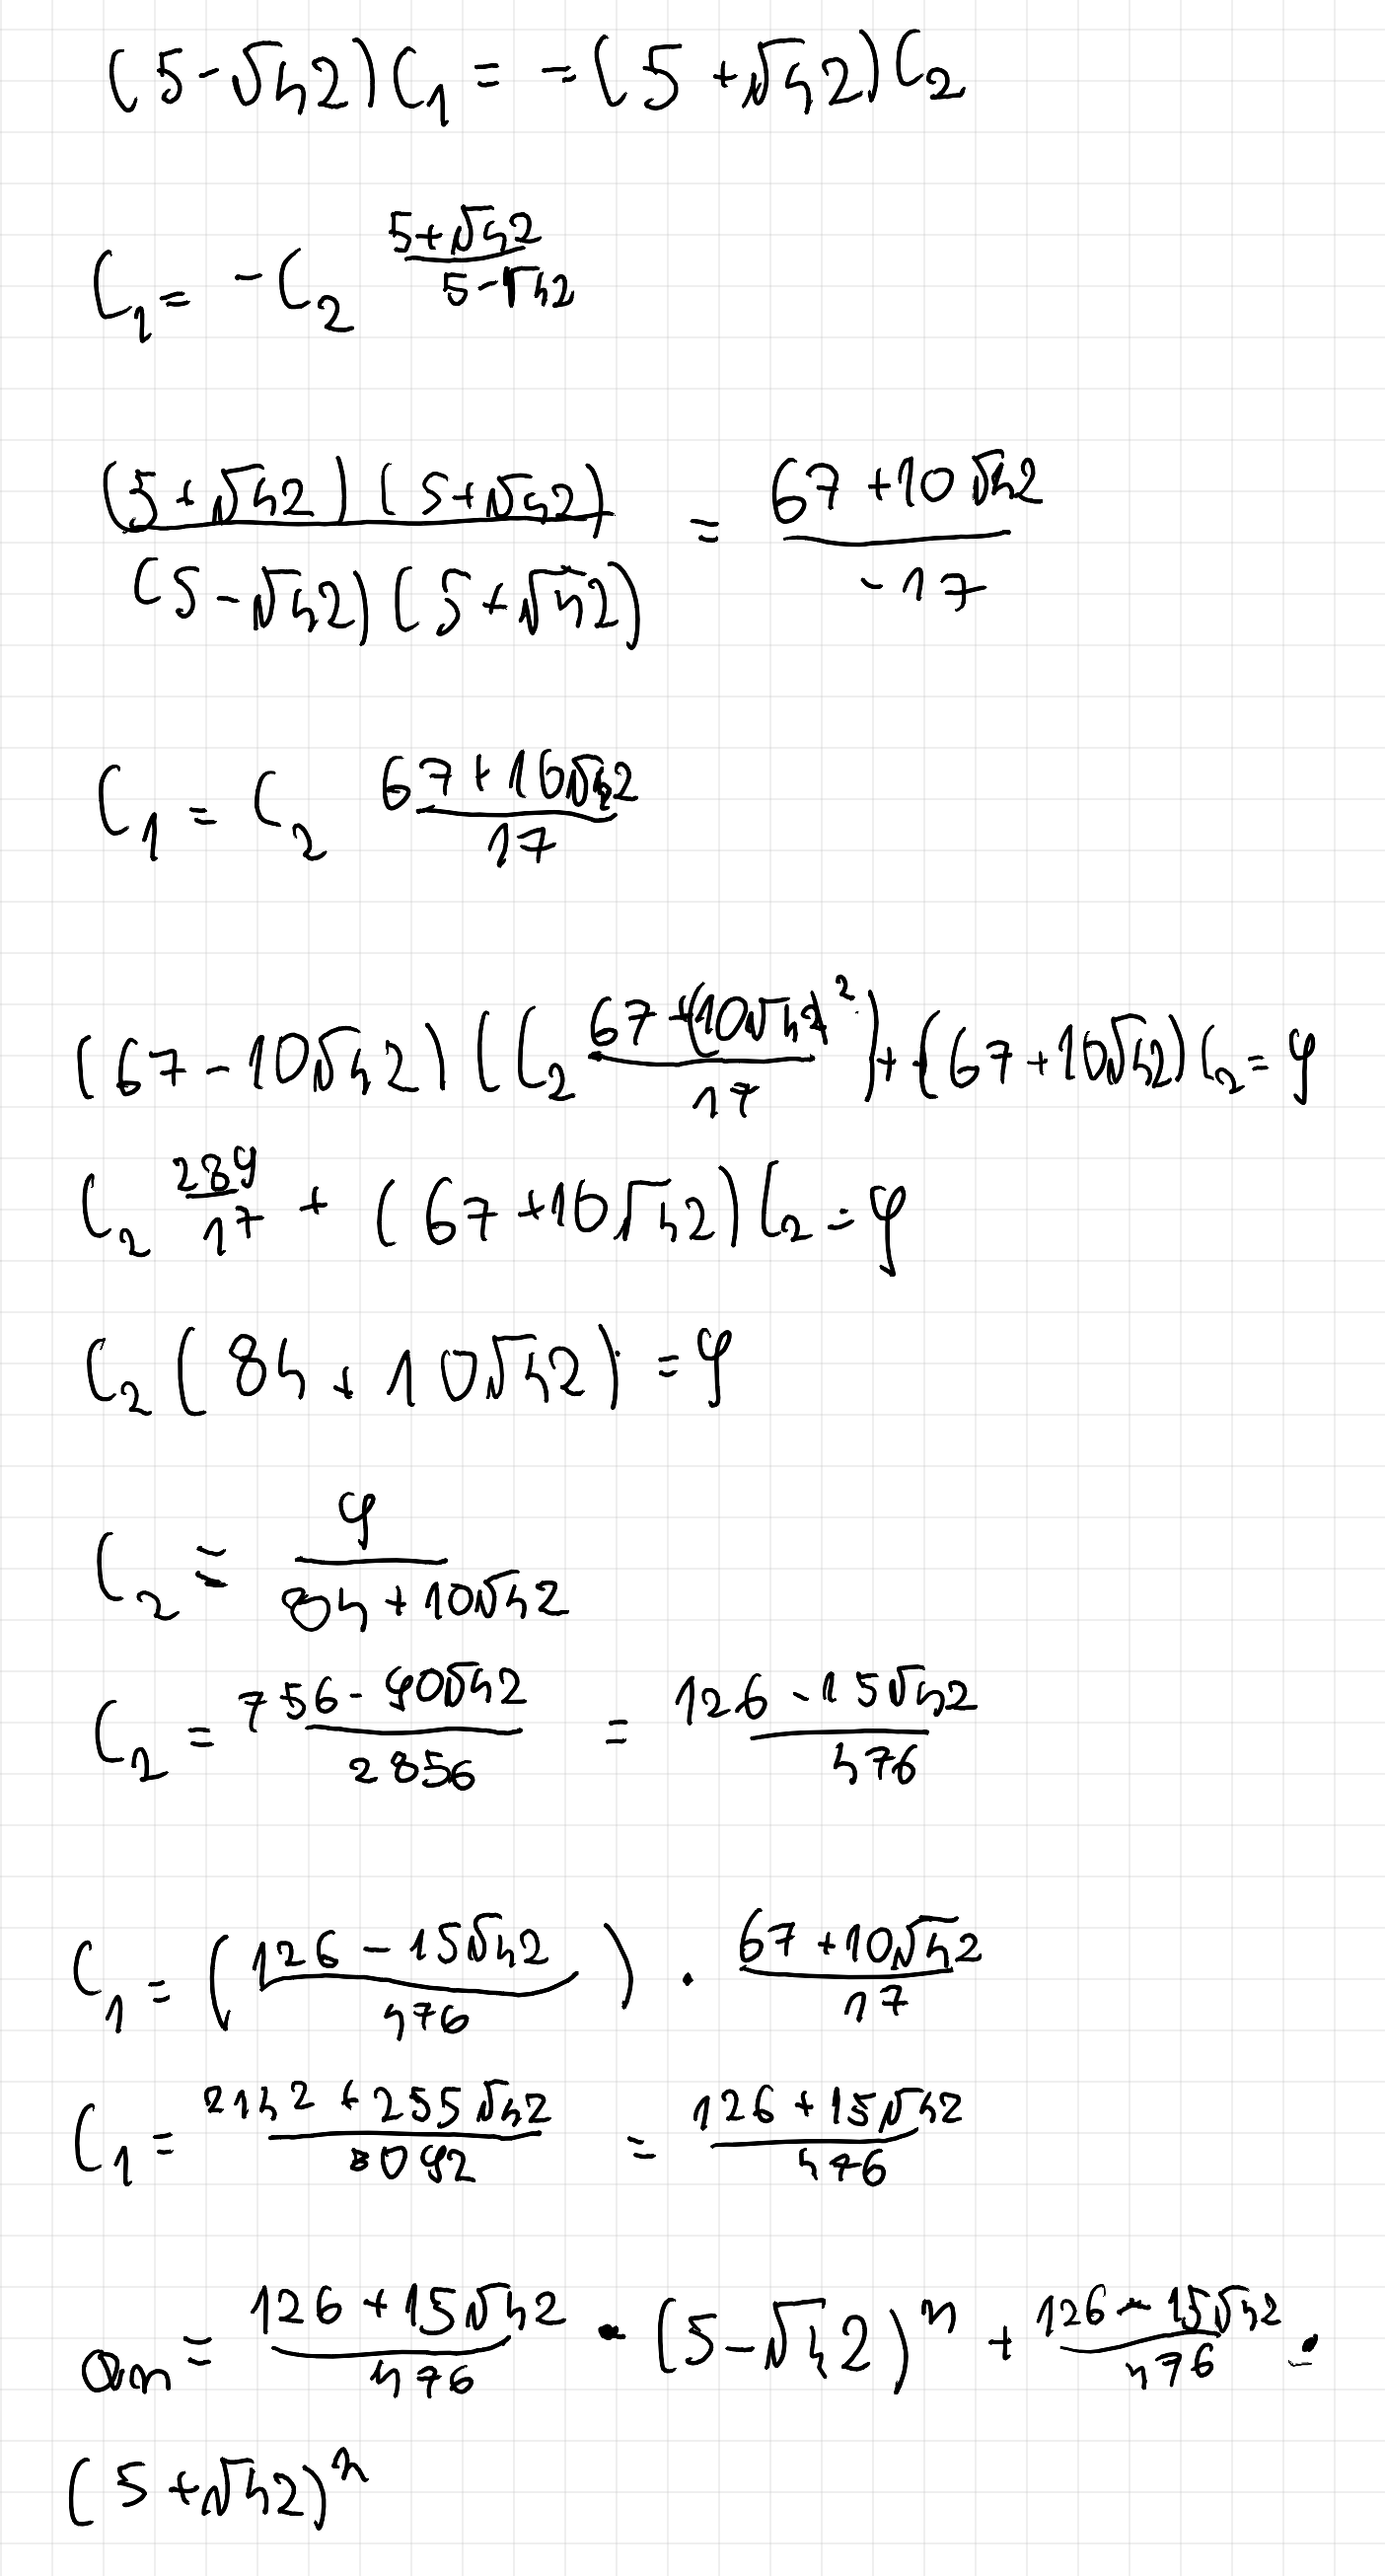
\includegraphics[width=0.65\textwidth]{jednorodne2.png}
    \caption{Wyznaczenie stałych i ostateczny wzór jawny ciągu.}
    \label{fig:jednorodne_2}
\end{figure}

\textbf{Opis do Rysunku \ref{fig:jednorodne_2}:}
Druga część obliczeń przedstawia żmudny proces algebraicznego rozwiązywania układu równań. Wykorzystano metodę podstawiania, wyznaczając $C_1$ w zależności od $C_2$, co ostatecznie pozwoliło na obliczenie dokładnych wartości obu stałych. Na samym dole zapisano końcowy, jawny wzór na n-ty wyraz ciągu $a_n$.

\begin{figure}[H]
    \centering
    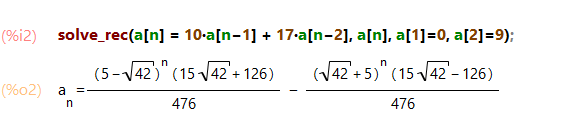
\includegraphics[width=0.85\textwidth]{maxima_jednorodne.png}
    \caption{Weryfikacja rozwiązania jednorodnego w programie Maxima.}
    \label{fig:jednorodne_maxima}
\end{figure}

\textbf{Opis do Rysunku \ref{fig:jednorodne_maxima}:}
Powyższy zrzut ekranu prezentuje wywołanie funkcji \texttt{solve\_rec} w systemie Maxima. Otrzymany wynik zgadza się z wartościami wyznaczonymi analitycznie, co potwierdza poprawność przeprowadzonych przekształceń.

\clearpage

\section{Równanie rekurencyjne niejednorodne}

W drugim kroku analizowano równanie rekurencyjne niejednorodne:
\begin{equation}
    a_n = 13a_{n-1} - 30a_{n-2} - n \cdot 10^n + 2 - 3^n
\end{equation}
z warunkami początkowymi $a_0 = 2$ oraz $a_1 = 5$. Z uwagi na stopień skomplikowania, obliczenia podzielono na trzy etapy.

\begin{figure}[H]
    \centering
    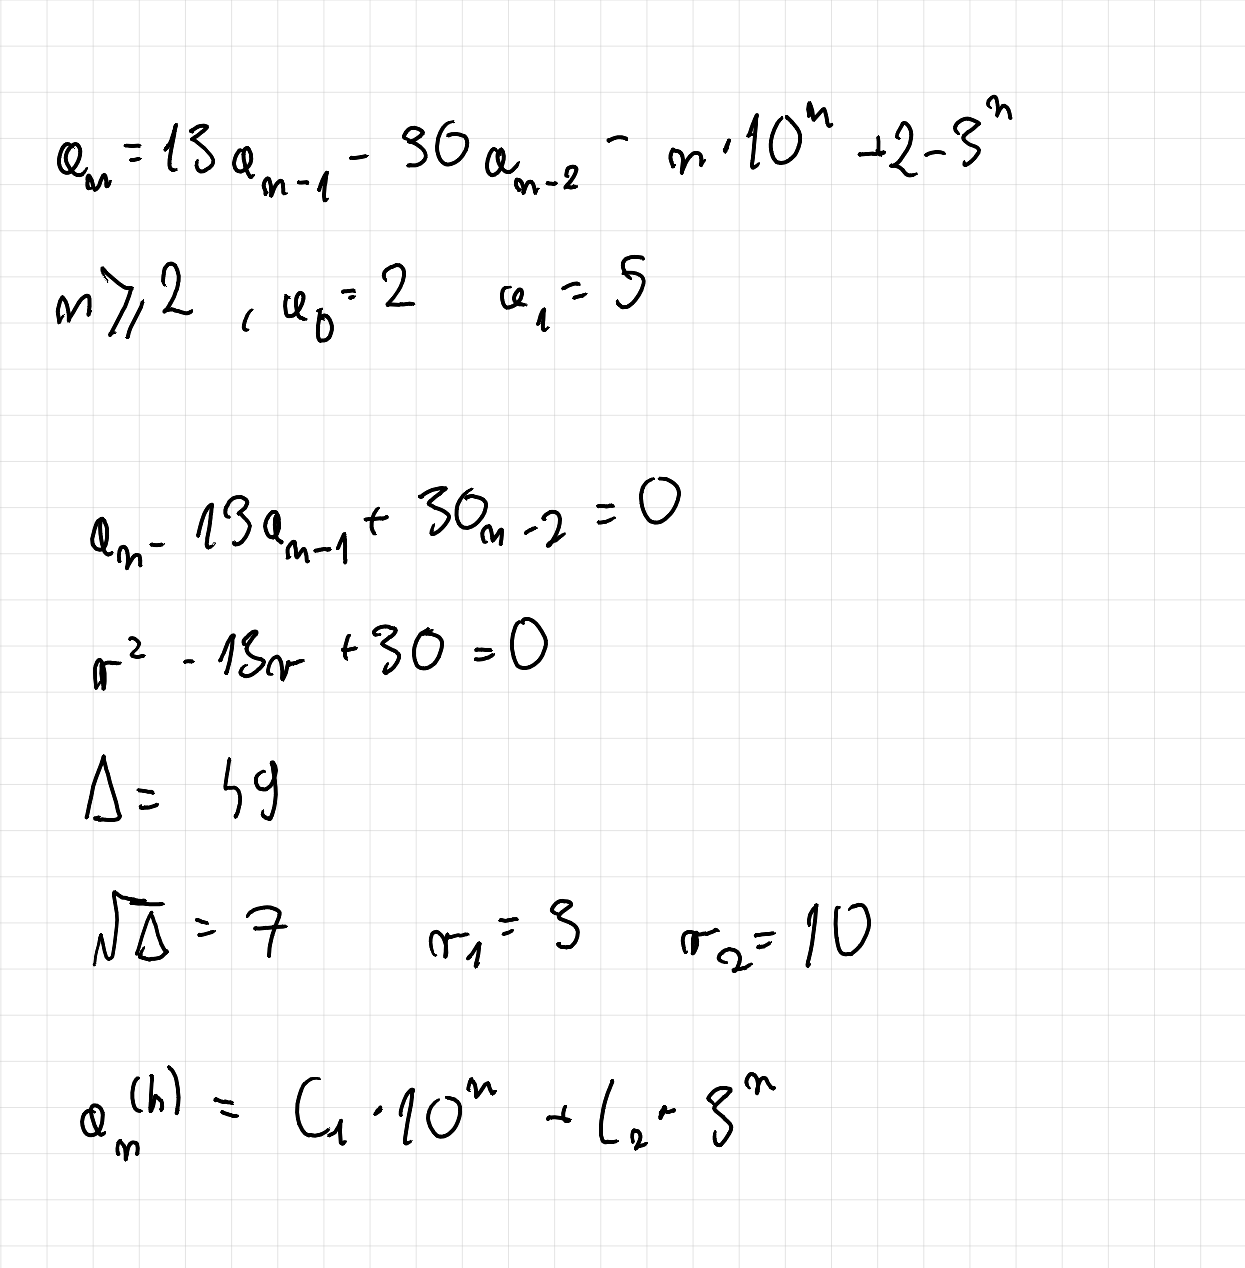
\includegraphics[width=0.6\textwidth]{niejednorodne.png}
    \caption{Rozwiązanie równania jednorodnego powiązanego z niejednorodnym.}
    \label{fig:niejednorodne_1}
\end{figure}

\textbf{Opis do Rysunku \ref{fig:niejednorodne_1}:}
Rozpoczęto od rozwiązania tzw. równania jednorodnego. Równanie charakterystyczne $r^2 - 13r + 30 = 0$ posiada pierwiastki $r_1 = 3$ i $r_2 = 10$. Dało to bazę do zbudowania ogólnego rozwiązania części jednorodnej: $a_n^{(h)} = C_1 \cdot 10^n + C_2 \cdot 3^n$.

\begin{figure}[H]
    \centering
    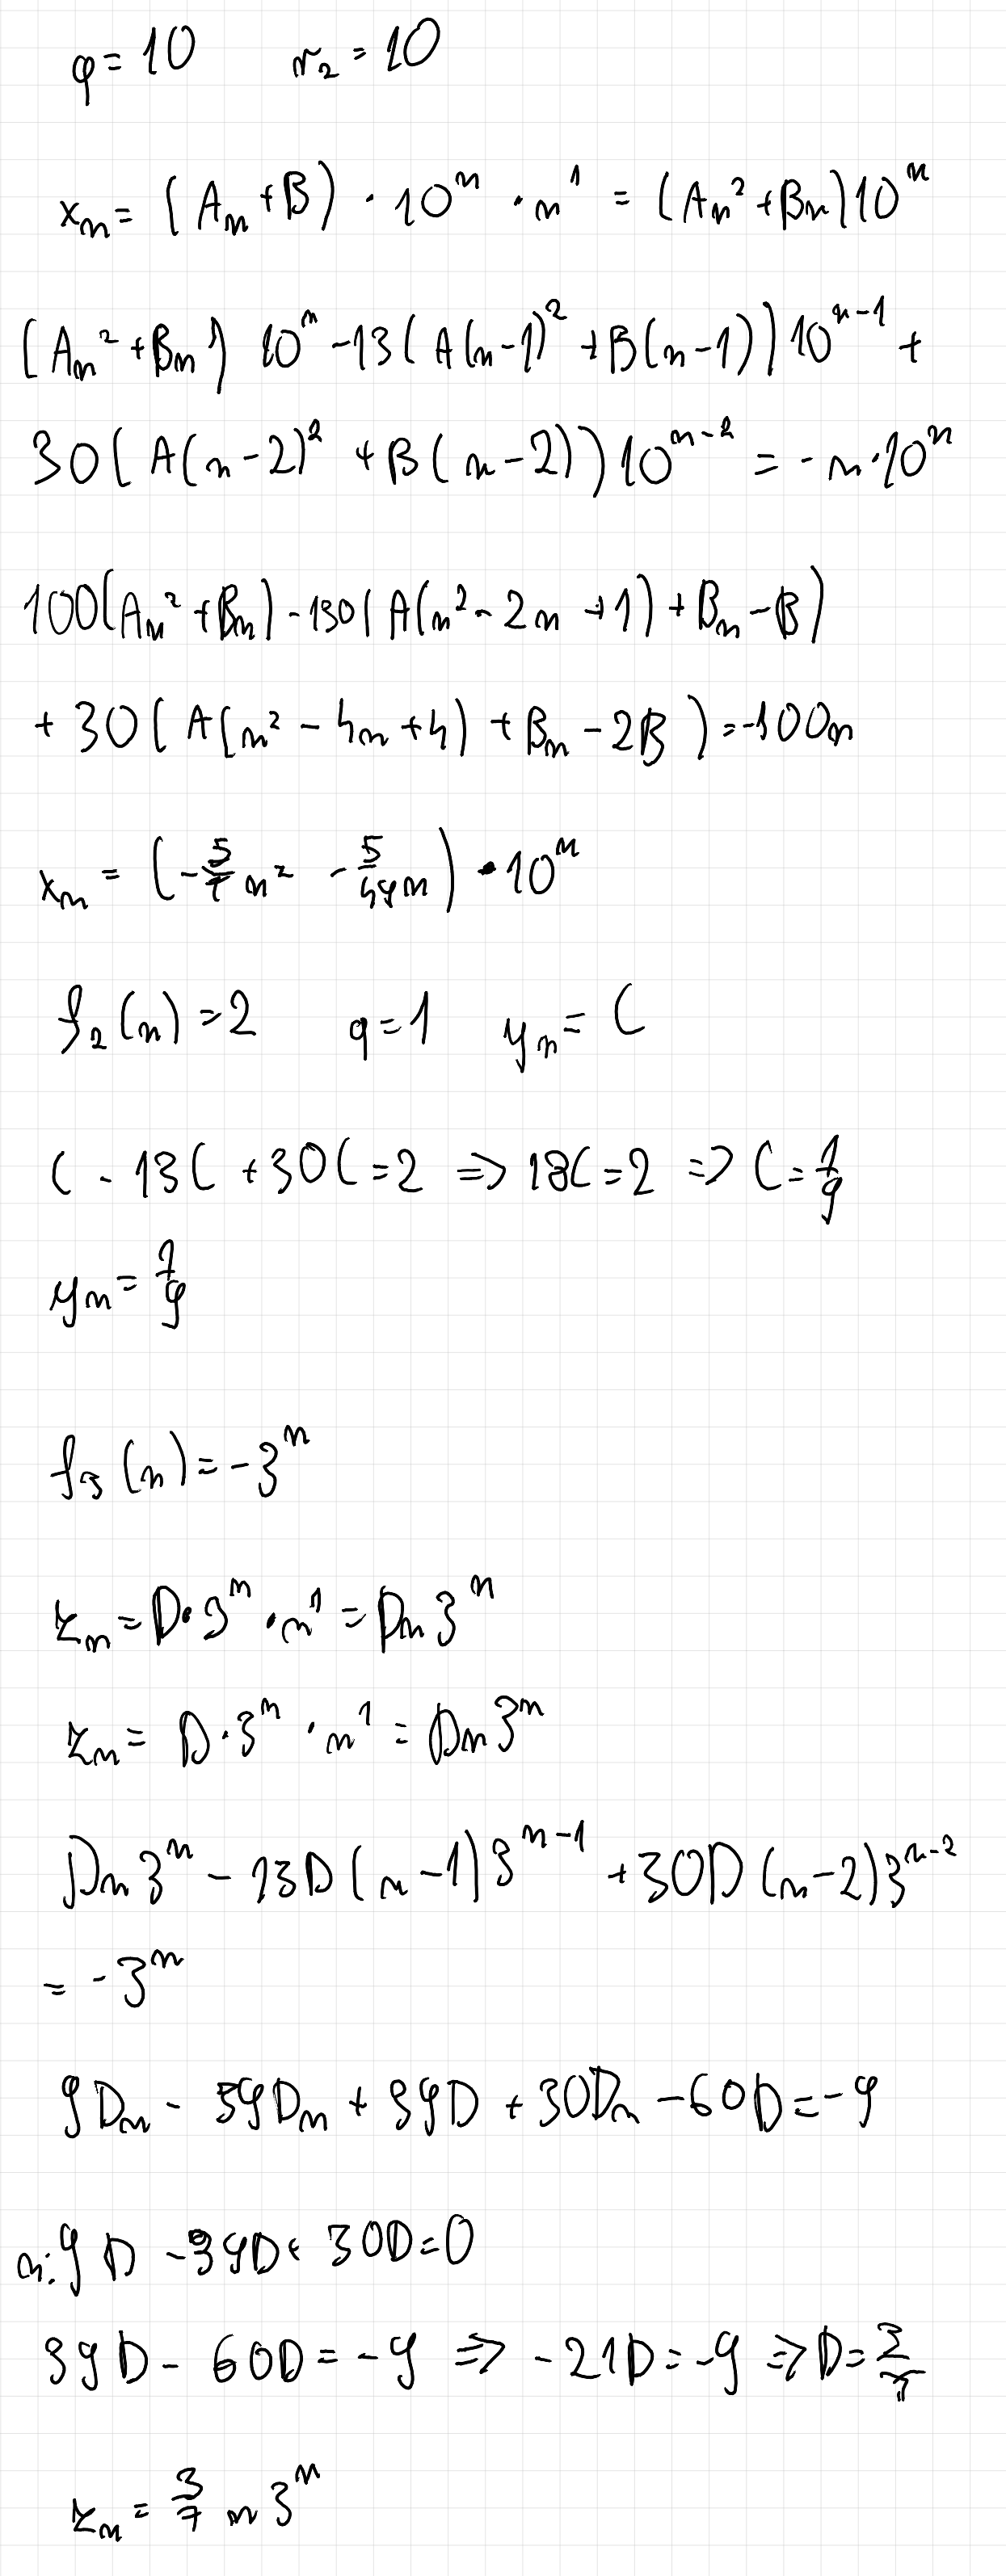
\includegraphics[width=0.45\textwidth]{niejednorodne2.png}
    \caption{Wyznaczanie rozwiązań szczególnych metodą przewidywań (część 1).}
    \label{fig:niejednorodne_2}
\end{figure}

\textbf{Opis do Rysunku \ref{fig:niejednorodne_2}:}
Na tym etapie zastosowano metodę współczynników nieoznaczonych (metodę przewidywań) dla prawej strony równania. Ze względu na to, że wartości $10$ oraz $3$ w części niejednorodnej pokrywają się z pierwiastkami równania charakterystycznego (przypadek rezonansu), przewidywane rozwiązania szczególne trzeba było pomnożyć przez dodatkowe $n$. Pokazano tu proces wyznaczania współczynników dla części wielomianowo-wykładniczej oraz dla stałej (gdzie wyliczono $C = \frac{1}{9}$).

\begin{figure}[H]
    \centering
    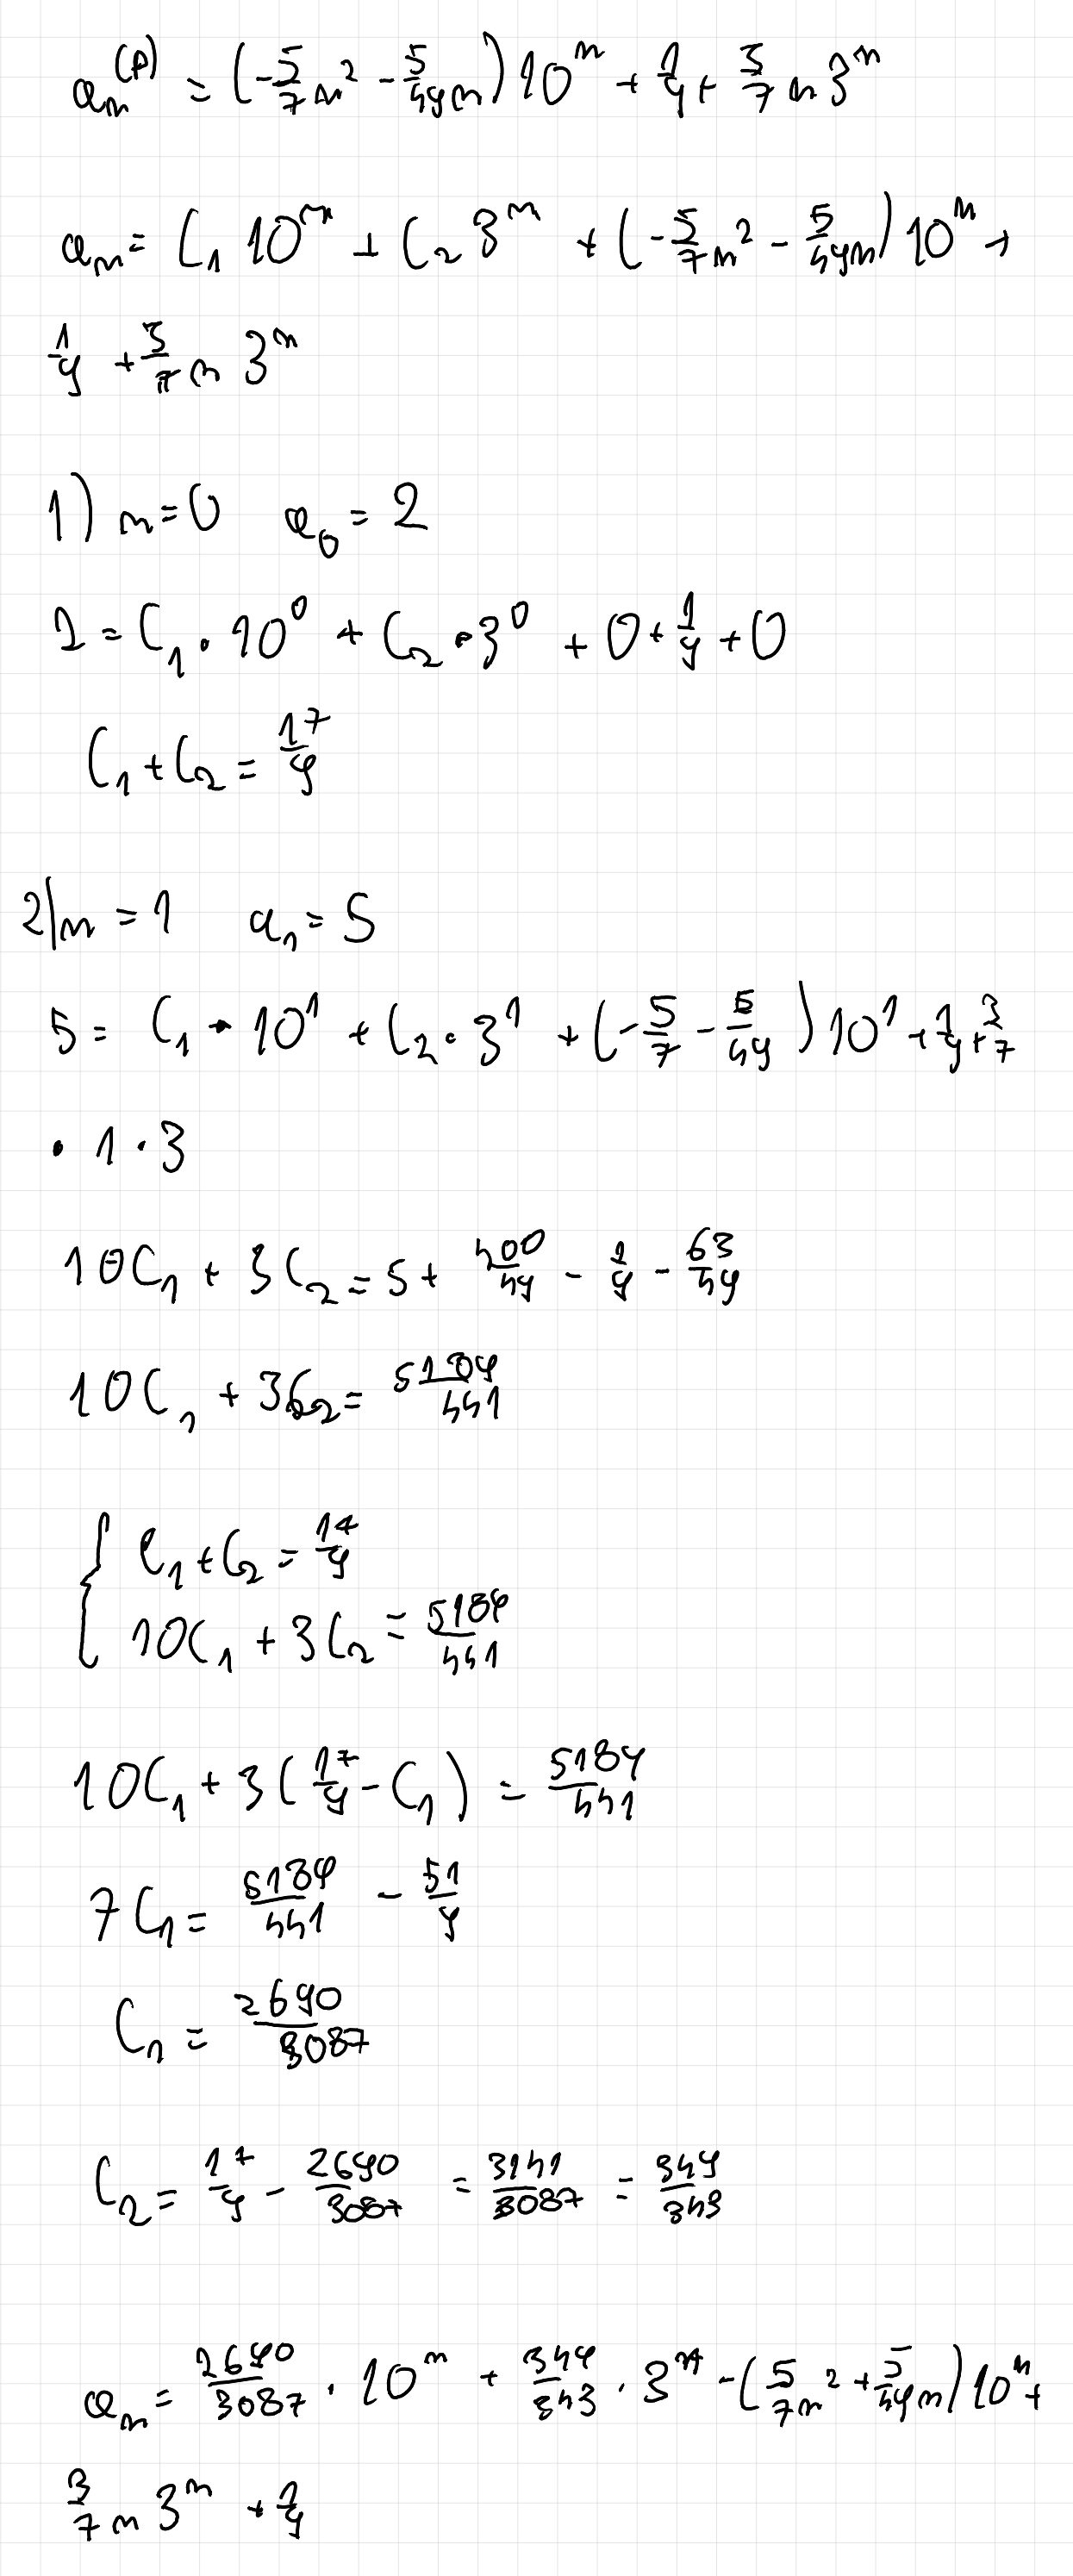
\includegraphics[width=0.45\textwidth]{niejednorodne3.png}
    \caption{Dokończenie metody przewidywań, uwzględnienie warunków początkowych i wynik końcowy.}
    \label{fig:niejednorodne_3}
\end{figure}

\textbf{Opis do Rysunku \ref{fig:niejednorodne_3}:}
Zdjęcie ukazuje dokończenie poszukiwań rozwiązania szczególnego dla elementu $-3^n$ (wyliczono stałą $D$). Następnie zsumowano wszystkie wyznaczone elementy, tworząc pełne rozwiązanie ogólne. Podstawiono warunki początkowe $a_0 = 2$ i $a_1 = 5$, zbudowano układ równań dla wyznaczenia głównych stałych $C_1$ i $C_2$, a na dole przedstawiono skomplikowany wzór jawny kończący zadanie.

\begin{figure}[H]
    \centering
    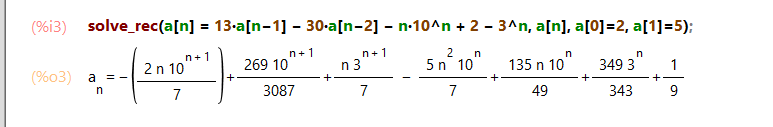
\includegraphics[width=0.9\textwidth]{maxima_niejednorodne.png}
    \caption{Weryfikacja rozwiązania niejednorodnego w programie Maxima.}
    \label{fig:niejednorodne_maxima}
\end{figure}

\textbf{Opis do Rysunku \ref{fig:niejednorodne_maxima}:}
Wynik działania funkcji \texttt{solve\_rec} dla równania niejednorodnego w programie Maxima. Złożony ułamek wygenerowany przez program potwierdza długie rachunki ręczne przeprowadzone w poprzednich krokach.

\subsection{Wizualizacja ciągu}

\begin{figure}[H]
    \centering
    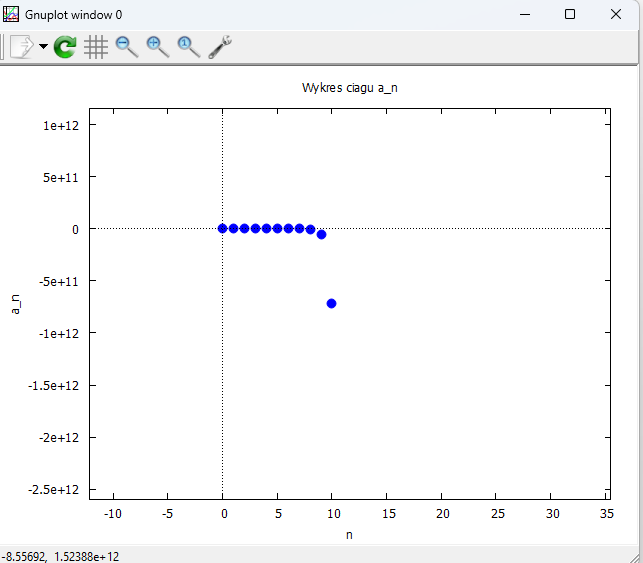
\includegraphics[width=0.7\textwidth]{niejednorodne_wykres.png}
    \caption{Wykres wartości wyrazów ciągu wygenerowany w Gnuplot.}
    \label{fig:wykres}
\end{figure}

\textbf{Opis do Rysunku \ref{fig:wykres}:}
Wykres punktowy wartości ciągu dla początkowych wyrazów $n$. Ze względu na obecność bardzo szybko rosnących i ujemnych czynników (np. pochodzących od elementu z potęgą $10^n$), wartości ciągu błyskawicznie "uciekają" w dół. Na wykresie widać, że już w okolicach $n=10$ ciąg osiąga gigantyczne wartości ujemne rzędu $-10^{12}$.

\section{Podsumowanie}
Rozwiązanie obu równań powiodło się, a ręczne metody analityczne zostały pozytywnie zweryfikowane. Podział obliczeń na etapy pokazał, jak złożony algorytmicznie jest to proces dla równań niejednorodnych w przypadku tzw. rezonansu (pokrywania się pierwiastków z częścią niejednorodną). Systemy takie jak Maxima okazały się nieocenione przy sprawdzaniu ostatecznego wyniku.

\end{document}